% Options for packages loaded elsewhere
\PassOptionsToPackage{unicode}{hyperref}
\PassOptionsToPackage{hyphens}{url}
%
\documentclass[
]{article}
\usepackage{lmodern}
\usepackage{amssymb,amsmath}
\usepackage{ifxetex,ifluatex}
\ifnum 0\ifxetex 1\fi\ifluatex 1\fi=0 % if pdftex
  \usepackage[T1]{fontenc}
  \usepackage[utf8]{inputenc}
  \usepackage{textcomp} % provide euro and other symbols
\else % if luatex or xetex
  \usepackage{unicode-math}
  \defaultfontfeatures{Scale=MatchLowercase}
  \defaultfontfeatures[\rmfamily]{Ligatures=TeX,Scale=1}
\fi
% Use upquote if available, for straight quotes in verbatim environments
\IfFileExists{upquote.sty}{\usepackage{upquote}}{}
\IfFileExists{microtype.sty}{% use microtype if available
  \usepackage[]{microtype}
  \UseMicrotypeSet[protrusion]{basicmath} % disable protrusion for tt fonts
}{}
\makeatletter
\@ifundefined{KOMAClassName}{% if non-KOMA class
  \IfFileExists{parskip.sty}{%
    \usepackage{parskip}
  }{% else
    \setlength{\parindent}{0pt}
    \setlength{\parskip}{6pt plus 2pt minus 1pt}}
}{% if KOMA class
  \KOMAoptions{parskip=half}}
\makeatother
\usepackage{xcolor}
\IfFileExists{xurl.sty}{\usepackage{xurl}}{} % add URL line breaks if available
\IfFileExists{bookmark.sty}{\usepackage{bookmark}}{\usepackage{hyperref}}
\hypersetup{
  pdftitle={Compilation de données : R Markdown \& GitHub},
  pdfauthor={Groupe 2 : Louise, Zélie, Paul, Juliette, Charlène, Axel},
  hidelinks,
  pdfcreator={LaTeX via pandoc}}
\urlstyle{same} % disable monospaced font for URLs
\usepackage[margin=1in]{geometry}
\usepackage{color}
\usepackage{fancyvrb}
\newcommand{\VerbBar}{|}
\newcommand{\VERB}{\Verb[commandchars=\\\{\}]}
\DefineVerbatimEnvironment{Highlighting}{Verbatim}{commandchars=\\\{\}}
% Add ',fontsize=\small' for more characters per line
\usepackage{framed}
\definecolor{shadecolor}{RGB}{248,248,248}
\newenvironment{Shaded}{\begin{snugshade}}{\end{snugshade}}
\newcommand{\AlertTok}[1]{\textcolor[rgb]{0.94,0.16,0.16}{#1}}
\newcommand{\AnnotationTok}[1]{\textcolor[rgb]{0.56,0.35,0.01}{\textbf{\textit{#1}}}}
\newcommand{\AttributeTok}[1]{\textcolor[rgb]{0.77,0.63,0.00}{#1}}
\newcommand{\BaseNTok}[1]{\textcolor[rgb]{0.00,0.00,0.81}{#1}}
\newcommand{\BuiltInTok}[1]{#1}
\newcommand{\CharTok}[1]{\textcolor[rgb]{0.31,0.60,0.02}{#1}}
\newcommand{\CommentTok}[1]{\textcolor[rgb]{0.56,0.35,0.01}{\textit{#1}}}
\newcommand{\CommentVarTok}[1]{\textcolor[rgb]{0.56,0.35,0.01}{\textbf{\textit{#1}}}}
\newcommand{\ConstantTok}[1]{\textcolor[rgb]{0.00,0.00,0.00}{#1}}
\newcommand{\ControlFlowTok}[1]{\textcolor[rgb]{0.13,0.29,0.53}{\textbf{#1}}}
\newcommand{\DataTypeTok}[1]{\textcolor[rgb]{0.13,0.29,0.53}{#1}}
\newcommand{\DecValTok}[1]{\textcolor[rgb]{0.00,0.00,0.81}{#1}}
\newcommand{\DocumentationTok}[1]{\textcolor[rgb]{0.56,0.35,0.01}{\textbf{\textit{#1}}}}
\newcommand{\ErrorTok}[1]{\textcolor[rgb]{0.64,0.00,0.00}{\textbf{#1}}}
\newcommand{\ExtensionTok}[1]{#1}
\newcommand{\FloatTok}[1]{\textcolor[rgb]{0.00,0.00,0.81}{#1}}
\newcommand{\FunctionTok}[1]{\textcolor[rgb]{0.00,0.00,0.00}{#1}}
\newcommand{\ImportTok}[1]{#1}
\newcommand{\InformationTok}[1]{\textcolor[rgb]{0.56,0.35,0.01}{\textbf{\textit{#1}}}}
\newcommand{\KeywordTok}[1]{\textcolor[rgb]{0.13,0.29,0.53}{\textbf{#1}}}
\newcommand{\NormalTok}[1]{#1}
\newcommand{\OperatorTok}[1]{\textcolor[rgb]{0.81,0.36,0.00}{\textbf{#1}}}
\newcommand{\OtherTok}[1]{\textcolor[rgb]{0.56,0.35,0.01}{#1}}
\newcommand{\PreprocessorTok}[1]{\textcolor[rgb]{0.56,0.35,0.01}{\textit{#1}}}
\newcommand{\RegionMarkerTok}[1]{#1}
\newcommand{\SpecialCharTok}[1]{\textcolor[rgb]{0.00,0.00,0.00}{#1}}
\newcommand{\SpecialStringTok}[1]{\textcolor[rgb]{0.31,0.60,0.02}{#1}}
\newcommand{\StringTok}[1]{\textcolor[rgb]{0.31,0.60,0.02}{#1}}
\newcommand{\VariableTok}[1]{\textcolor[rgb]{0.00,0.00,0.00}{#1}}
\newcommand{\VerbatimStringTok}[1]{\textcolor[rgb]{0.31,0.60,0.02}{#1}}
\newcommand{\WarningTok}[1]{\textcolor[rgb]{0.56,0.35,0.01}{\textbf{\textit{#1}}}}
\usepackage{graphicx,grffile}
\makeatletter
\def\maxwidth{\ifdim\Gin@nat@width>\linewidth\linewidth\else\Gin@nat@width\fi}
\def\maxheight{\ifdim\Gin@nat@height>\textheight\textheight\else\Gin@nat@height\fi}
\makeatother
% Scale images if necessary, so that they will not overflow the page
% margins by default, and it is still possible to overwrite the defaults
% using explicit options in \includegraphics[width, height, ...]{}
\setkeys{Gin}{width=\maxwidth,height=\maxheight,keepaspectratio}
% Set default figure placement to htbp
\makeatletter
\def\fps@figure{htbp}
\makeatother
\setlength{\emergencystretch}{3em} % prevent overfull lines
\providecommand{\tightlist}{%
  \setlength{\itemsep}{0pt}\setlength{\parskip}{0pt}}
\setcounter{secnumdepth}{5}

\title{Compilation de données : R Markdown \& GitHub}
\author{Groupe 2 : Louise, Zélie, Paul, Juliette, Charlène, Axel}
\date{29/04/20}

\begin{document}
\maketitle

{
\setcounter{tocdepth}{3}
\tableofcontents
}
\begin{figure}[h]

{\centering 
\includegraphics[width=0.8\linewidth]{rmarkdown} 

}

\caption{Logo Rmarkdown}\label{fig:logo}
\end{figure}

~

\textbf{Résumé} : Dans ce rapport nous analyserons les temperatures des
principales villes françaises.\\
\ldots\ldots\ldots\ldots\ldots\ldots\ldots\ldots\ldots\ldots\ldots\ldots\ldots\ldots\ldots\ldots\ldots\ldots\ldots\ldots\ldots\ldots\ldots\ldots\ldots\ldots\ldots\ldots\ldots\ldots\ldots\ldots\ldots\ldots\ldots\ldots\ldots\ldots{}
\ldots\ldots\ldots\ldots\ldots\ldots\ldots\ldots\ldots\ldots\ldots\ldots\ldots\ldots\ldots\ldots\ldots\ldots\ldots\ldots\ldots\ldots\ldots\ldots\ldots\ldots\ldots\ldots\ldots\ldots\ldots\ldots\ldots\ldots\ldots\ldots\ldots\ldots{}

~

\hypertarget{pruxe9sentation-des-donnuxe9es}{%
\section{\texorpdfstring{\textbf{Présentation des données
}}{Présentation des données }}\label{pruxe9sentation-des-donnuxe9es}}

Les données sont téléchargeables directement sur
\href{https://husson.github.io/data.html}{ce site} ou peuvent être
importée directement sous R avec :

\begin{Shaded}
\begin{Highlighting}[]
\NormalTok{link <-}\StringTok{ "http://factominer.free.fr/course/donnees/AnaDo_JeuDonnees_TemperatFrance.csv"}
\NormalTok{datatemp <-}\StringTok{ }\KeywordTok{read.table}\NormalTok{(link, }\DataTypeTok{h=}\OtherTok{TRUE}\NormalTok{, }\DataTypeTok{sep=}\StringTok{";"}\NormalTok{, }\DataTypeTok{dec=}\StringTok{"."}\NormalTok{, }\DataTypeTok{row.names=}\DecValTok{1}\NormalTok{, }\DataTypeTok{encoding=}\StringTok{"latin1"}\NormalTok{)}
\CommentTok{##dd <- as_tibble(datatemp)}
\end{Highlighting}
\end{Shaded}

\hypertarget{les-donnuxe9es}{%
\subsection{\texorpdfstring{\textbf{Les
données}}{Les données}}\label{les-donnuxe9es}}

\begin{verbatim}
##          Janv Févr Mars Avri  Mai Juin juil Août Sept Octo Nove Déce  Lati
## Bordeaux  5.6  6.6 10.3 12.8 15.8 19.3 20.9 21.0 18.6 13.8  9.1  6.2 44.50
## Brest     6.1  5.8  7.8  9.2 11.6 14.4 15.6 16.0 14.7 12.0  9.0  7.0 48.24
## Clermont  2.6  3.7  7.5 10.3 13.8 17.3 19.4 19.1 16.2 11.2  6.6  3.6 45.47
## Grenoble  1.5  3.2  7.7 10.6 14.5 17.8 20.1 19.5 16.7 11.4  6.5  2.3 45.10
## Lille     2.4  2.9  6.0  8.9 12.4 15.3 17.1 17.1 14.7 10.4  6.1  3.5 50.38
## Lyon      2.1  3.3  7.7 10.9 14.9 18.5 20.7 20.1 16.9 11.4  6.7  3.1 45.45
##           Long  Moye Ampl Région
## Bordeaux -0.34 13.33 15.4     SO
## Brest    -4.29 10.77 10.2     NO
## Clermont  3.05 10.94 16.8     SE
## Grenoble  5.43 10.98 18.6     SE
## Lille     3.04  9.73 14.7     NE
## Lyon      4.51 11.36 18.6     SE
\end{verbatim}

~

Le jeu de donné est complété pour 15 villes et contient 17 variables
dont les tempértures des 12 mois de l'année, la moyenne, l'amplitude,
latitude et longitude ainsi qu'un indicateur de grandes régions. La
temperature moyenne en France est égale à 11.81 \(+/-\) 5.93 degrés
Celcius (moyenne \(+/-\) écart type). La ville la plus froide est :
Strasbourg ; et la ville la plus chaudes est : Nice (Fig.
\textbackslash ref\{fig:\{tempvilles\}).

\begin{figure}[h]

{\centering 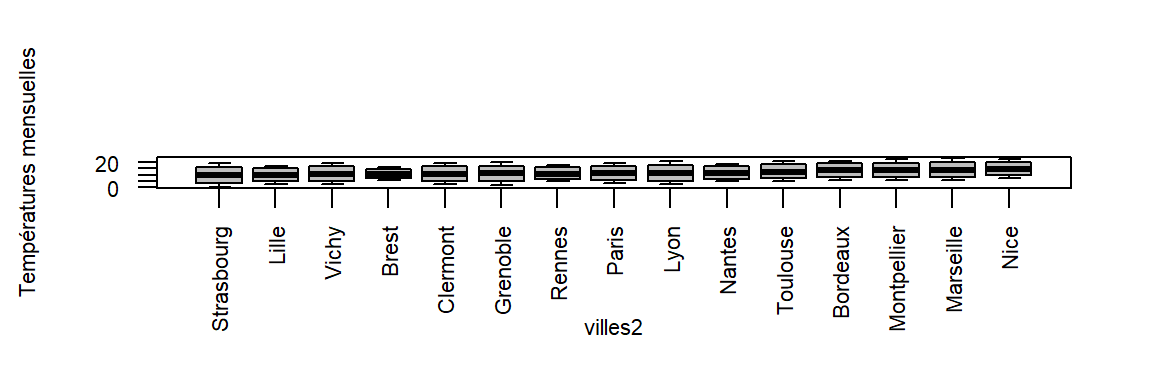
\includegraphics{rapport_bad2_files/figure-latex/datatempville-1} 

}

\caption{Températures par villes\label{fig:tempvilles}}\label{fig:datatempville}
\end{figure}

~

\hypertarget{une-premiuxe8re-analyse}{%
\section{\texorpdfstring{\textbf{Une première analyse
}}{Une première analyse }}\label{une-premiuxe8re-analyse}}

Nous réalisons des graphiques permettant d'analyser, par région :

\begin{itemize}
\item
  La position globale de la températures vis à vis de la moyenne
  nationale.

  L'évolution mensuelle des températures dont notament :

  L'amplitude

  \begin{itemize}
  \tightlist
  \item
    L'hétérogénéité inter-villes.
  \end{itemize}
\end{itemize}

\hypertarget{cruxe9ation-dune-fonction-graphique}{%
\subsection{\texorpdfstring{\textbf{Création d'une fonction
graphique}}{Création d'une fonction graphique}}\label{cruxe9ation-dune-fonction-graphique}}

Nous souhaitons produire un graphique representant par région les
courbes mensuelles de chaque ville avec la courbe moyenne nationale.
Voici un script possible :

\begin{Shaded}
\begin{Highlighting}[]
\NormalTok{Tplot<-}\ControlFlowTok{function}\NormalTok{(tempr,tmean) \{}
  \KeywordTok{plot}\NormalTok{(}\KeywordTok{c}\NormalTok{(}\DecValTok{1}\NormalTok{,}\DecValTok{12}\NormalTok{),}\KeywordTok{c}\NormalTok{(}\OperatorTok{-}\DecValTok{10}\NormalTok{,}\DecValTok{30}\NormalTok{),}\DataTypeTok{type=}\StringTok{"n"}\NormalTok{,}\DataTypeTok{ylab=}\StringTok{"Temperature (°C)"}\NormalTok{,}\DataTypeTok{xlab=}\StringTok{"Mois"}\NormalTok{,}\DataTypeTok{cex.lab=}\FloatTok{0.8}\NormalTok{,}\DataTypeTok{cex.axis=}\FloatTok{0.8}\NormalTok{)}
  \KeywordTok{apply}\NormalTok{(tempr[,}\DecValTok{1}\OperatorTok{:}\DecValTok{12}\NormalTok{],}\DecValTok{1}\NormalTok{,}\ControlFlowTok{function}\NormalTok{(x) }\KeywordTok{lines}\NormalTok{(}\DecValTok{1}\OperatorTok{:}\DecValTok{12}\NormalTok{,x))}
  \KeywordTok{text}\NormalTok{(}\DecValTok{2}\NormalTok{,}\DecValTok{28}\NormalTok{,tempr}\OperatorTok{$}\NormalTok{Région[}\DecValTok{1}\NormalTok{],}\DataTypeTok{cex=}\FloatTok{0.8}\NormalTok{)}
  \KeywordTok{lines}\NormalTok{(}\DecValTok{1}\OperatorTok{:}\DecValTok{12}\NormalTok{,tmean,}\DataTypeTok{lwd=}\DecValTok{2}\NormalTok{,}\DataTypeTok{col=}\StringTok{"red"}\NormalTok{)}
\NormalTok{\}}
\end{Highlighting}
\end{Shaded}

\hypertarget{application}{%
\subsection{\texorpdfstring{\emph{Application}}{Application}}\label{application}}

\begin{Shaded}
\begin{Highlighting}[]
\CommentTok{#température moyenne}
\NormalTok{tmean<-}\KeywordTok{apply}\NormalTok{(datatemp[,}\DecValTok{1}\OperatorTok{:}\DecValTok{12}\NormalTok{],}\DecValTok{2}\NormalTok{,mean)}
\CommentTok{#Découpage du tableau par région}
\NormalTok{sptemp<-}\KeywordTok{split}\NormalTok{(datatemp,datatemp}\OperatorTok{$}\NormalTok{Région)}
\CommentTok{#Découpage de la fenêtre graphique}
\KeywordTok{par}\NormalTok{(}\DataTypeTok{mfrow=}\KeywordTok{c}\NormalTok{(}\DecValTok{2}\NormalTok{,}\DecValTok{2}\NormalTok{),}\DataTypeTok{mar=}\KeywordTok{c}\NormalTok{(}\DecValTok{3}\NormalTok{,}\DecValTok{3}\NormalTok{,}\DecValTok{1}\NormalTok{,}\DecValTok{1}\NormalTok{),}\DataTypeTok{mgp=}\KeywordTok{c}\NormalTok{(}\DecValTok{2}\NormalTok{,}\DecValTok{1}\NormalTok{,}\DecValTok{0}\NormalTok{))}
\CommentTok{#Application de la fonction}
\NormalTok{plot<-}\KeywordTok{lapply}\NormalTok{(sptemp,Tplot,tmean)}
\CommentTok{#Légende}
\KeywordTok{legend}\NormalTok{(}\DecValTok{4}\NormalTok{,}\DecValTok{0}\NormalTok{,}\StringTok{"Moyennes nationales"}\NormalTok{,}\DataTypeTok{bty=}\StringTok{"n"}\NormalTok{,}\DataTypeTok{col=}\StringTok{"red"}\NormalTok{,}\DataTypeTok{lwd=}\DecValTok{2}\NormalTok{,}\DataTypeTok{cex=}\FloatTok{0.7}\NormalTok{)}
\end{Highlighting}
\end{Shaded}

\begin{figure}[h]

{\centering \includegraphics{rapport_bad2_files/figure-latex/graphtemp-1} 

}

\caption{Courbes de températures mensuelles par régions}\label{fig:graphtemp}
\end{figure}

\textbf{Interpretation}: Nous observons que
\ldots\ldots\ldots\ldots\ldots\ldots\ldots\ldots\ldots\ldots\ldots\ldots\ldots\ldots\ldots\ldots\ldots\ldots\ldots\ldots\ldots\ldots\ldots\ldots\ldots\ldots\ldots\ldots\ldots\ldots\ldots\ldots\ldots\ldots\ldots\ldots\ldots\ldots\ldots\ldots\ldots\ldots\ldots\ldots\ldots\ldots\ldots\ldots\ldots\ldots\ldots\ldots\ldots\ldots\ldots\ldots\ldots\ldots\ldots\ldots\ldots\ldots\ldots\ldots\ldots\ldots\ldots\ldots\ldots\ldots\ldots\ldots\ldots\ldots\ldots\ldots\ldots\ldots\ldots\ldots\ldots\ldots\ldots\ldots\ldots\ldots\ldots\ldots\ldots\ldots\ldots\ldots\ldots\ldots\ldots\ldots\ldots\ldots\ldots\ldots\ldots\ldots\ldots\ldots\ldots\ldots\ldots\ldots\ldots\ldots\ldots\ldots\ldots\ldots\ldots\ldots\ldots\ldots\ldots\ldots\ldots\ldots\ldots\ldots\ldots\ldots\ldots\ldots\ldots\ldots\ldots\ldots\ldots\ldots\ldots\ldots\ldots\ldots\ldots\ldots\ldots\ldots\ldots\ldots\ldots\ldots\ldots\ldots\ldots\ldots\ldots\ldots\ldots\ldots\ldots\ldots\ldots\ldots\ldots\ldots\ldots\ldots\ldots\ldots\ldots\ldots\ldots\ldots\ldots\ldots\ldots\ldots\ldots\ldots\ldots{}

~ \# \textbf{Analyse en Composante Principale}

\hypertarget{rappels}{%
\subsection{\texorpdfstring{\textbf{Rappels}}{Rappels}}\label{rappels}}

Une ACP permet d'analyser simulatnément les liens entre de multiples
variables quantitatives et d'analyser les positions des individus
statistiques vis à vis de l'ensemble de ces variables. Elle est basée
sur la recheches d'axes principaux indépendants, chacuns plus ou moins
liés aux variables d'entrées. Le première axe explique un maximum
d'intertie, le second une moindre partie et ainsi de suite. Pour rappel
l'intertie totale se calcul par :
\[I=\sum^N_{i=1}\frac{1}{N}d^2_{(e_i;g)}\] Avec :
\(d^2_{e_i,g}=\sum^p_{j=1}x^2_{ij}\) = Distance euclidienne au centre de
gravité du nuage de point (soit \((0;0)\)) avec des données centrée et
normées.

\hypertarget{les-valeurs-propres}{%
\subsection{\texorpdfstring{\textbf{Les valeurs
propres}}{Les valeurs propres}}\label{les-valeurs-propres}}

Elles permettent de determiner la proportion d'intertie expliquée par
chacuns des axes.

\begin{Shaded}
\begin{Highlighting}[]
\NormalTok{res <-}\StringTok{ }\KeywordTok{PCA}\NormalTok{(datatemp, }\DataTypeTok{quanti.sup=}\DecValTok{13}\OperatorTok{:}\DecValTok{16}\NormalTok{, }\DataTypeTok{quali.sup=}\DecValTok{17}\NormalTok{,}\DataTypeTok{graph=}\NormalTok{F)}
\KeywordTok{par}\NormalTok{(}\DataTypeTok{mfrow=}\KeywordTok{c}\NormalTok{(}\DecValTok{1}\NormalTok{,}\DecValTok{1}\NormalTok{),}\DataTypeTok{mar=}\KeywordTok{c}\NormalTok{(}\DecValTok{4}\NormalTok{,}\DecValTok{4}\NormalTok{,}\DecValTok{2}\NormalTok{,}\DecValTok{2}\NormalTok{))}
\KeywordTok{barplot}\NormalTok{(res}\OperatorTok{$}\NormalTok{eig[,}\DecValTok{2}\NormalTok{],}\DataTypeTok{ylab=}\StringTok{"Inertie %"}\NormalTok{,}\DataTypeTok{names.arg =} \KeywordTok{paste}\NormalTok{(}\StringTok{"Axe"}\NormalTok{,}\DecValTok{1}\OperatorTok{:}\StringTok{ }\KeywordTok{nrow}\NormalTok{(res}\OperatorTok{$}\NormalTok{eig)),}\DataTypeTok{las=}\DecValTok{2}\NormalTok{,}\DataTypeTok{cex.axis=}\FloatTok{0.7}\NormalTok{,}\DataTypeTok{cex.lab=}\FloatTok{0.8}\NormalTok{)}
\end{Highlighting}
\end{Shaded}

\begin{figure}[h]

{\centering \includegraphics{rapport_bad2_files/figure-latex/valp-1} 

}

\caption{Valeurs propres}\label{fig:valp}
\end{figure}

\textbf{Interpretation}: Nous observons que l'axe 1 explique 79.85\(\%\)
de l'intertie totale\\
\ldots\ldots\ldots\ldots\ldots\ldots\ldots\ldots\ldots\ldots\ldots\ldots\ldots\ldots\ldots\ldots\ldots\ldots\ldots\ldots\ldots\ldots\ldots\ldots\ldots\ldots\ldots\ldots\ldots\ldots\ldots\ldots\ldots\ldots\ldots\ldots\ldots\ldots{}
\ldots\ldots\ldots\ldots\ldots\ldots\ldots\ldots\ldots\ldots\ldots\ldots\ldots\ldots\ldots\ldots\ldots\ldots\ldots\ldots\ldots\ldots\ldots\ldots\ldots\ldots\ldots\ldots\ldots\ldots\ldots\ldots\ldots\ldots\ldots\ldots\ldots\ldots{}

\hypertarget{le-cercle-des-corruxe9lations}{%
\subsection{\texorpdfstring{\textbf{Le cercle des
corrélations}}{Le cercle des corrélations}}\label{le-cercle-des-corruxe9lations}}

\textbf{Interpretation}: Nous observons que l'axe 1 est expliqué par
\ldots\ldots\ldots\ldots\ldots\ldots\ldots\ldots\ldots\ldots\ldots\ldots\ldots\ldots\ldots\ldots\ldots\ldots.\\
\ldots\ldots\ldots\ldots\ldots\ldots\ldots\ldots\ldots\ldots\ldots\ldots\ldots\ldots\ldots\ldots\ldots\ldots\ldots\ldots\ldots\ldots\ldots\ldots\ldots\ldots\ldots\ldots\ldots\ldots\ldots\ldots\ldots\ldots\ldots\ldots\ldots\ldots{}
\ldots\ldots\ldots\ldots\ldots\ldots\ldots\ldots\ldots\ldots\ldots\ldots\ldots\ldots\ldots\ldots\ldots\ldots\ldots\ldots\ldots\ldots\ldots\ldots\ldots\ldots\ldots\ldots\ldots\ldots\ldots\ldots\ldots\ldots\ldots\ldots\ldots\ldots{}

\begin{Shaded}
\begin{Highlighting}[]
\KeywordTok{plot.PCA}\NormalTok{(res, }\DataTypeTok{choix=}\StringTok{"var"}\NormalTok{,}\DataTypeTok{cex.axis=}\FloatTok{0.7}\NormalTok{,}\DataTypeTok{cex.lab=}\FloatTok{0.8}\NormalTok{)}
\end{Highlighting}
\end{Shaded}

\begin{figure}[h]

{\centering \includegraphics{rapport_bad2_files/figure-latex/indiv-1} 

}

\caption{Cercle des corrélations}\label{fig:indiv}
\end{figure}

\hypertarget{le-nuage-des-individus}{%
\subsection{\texorpdfstring{\textbf{Le nuage des
individus}}{Le nuage des individus}}\label{le-nuage-des-individus}}

\begin{Shaded}
\begin{Highlighting}[]
\KeywordTok{plot.PCA}\NormalTok{(res, }\DataTypeTok{choix=}\StringTok{"ind"}\NormalTok{, }\DataTypeTok{habillage=}\DecValTok{17}\NormalTok{,}\DataTypeTok{cex.axis=}\FloatTok{0.7}\NormalTok{,}\DataTypeTok{cex.lab=}\FloatTok{0.8}\NormalTok{)}
\end{Highlighting}
\end{Shaded}

\begin{figure}[h]

{\centering \includegraphics{rapport_bad2_files/figure-latex/circle-1} 

}

\caption{Nuage des individus}\label{fig:circle}
\end{figure}

\textbf{Interpretation}: Nous observons que les villes du nord ouest se
caractérisent par\\
\ldots\ldots\ldots\ldots\ldots\ldots\ldots\ldots\ldots\ldots\ldots\ldots\ldots\ldots\ldots\ldots\ldots\ldots\ldots\ldots\ldots\ldots\ldots\ldots\ldots\ldots\ldots\ldots\ldots\ldots\ldots\ldots\ldots\ldots\ldots\ldots\ldots\ldots{}
\ldots\ldots\ldots\ldots\ldots\ldots\ldots\ldots\ldots\ldots\ldots\ldots\ldots\ldots\ldots\ldots\ldots\ldots\ldots\ldots\ldots\ldots\ldots\ldots\ldots\ldots\ldots\ldots\ldots\ldots\ldots\ldots\ldots\ldots\ldots\ldots\ldots\ldots{}
\ldots\ldots\ldots\ldots\ldots\ldots\ldots\ldots\ldots\ldots\ldots\ldots\ldots\ldots\ldots\ldots\ldots\ldots\ldots\ldots\ldots\ldots\ldots\ldots\ldots\ldots\ldots\ldots\ldots\ldots\ldots\ldots\ldots\ldots\ldots\ldots\ldots\ldots{}

~

\hypertarget{conclusions}{%
\subsection{\texorpdfstring{\textbf{Conclusions
}}{Conclusions }}\label{conclusions}}

Les variations mensuelles des température semblent être liées aux
différents climats existants en France et plus largement en Europe
(Rebetez et al., 2006). Néanmoins la France est soumise à des
changements climatiques (passés, ex : Moisselin et al., 2002~; et
présents, ex : Lespinas et al., 2010). Ceci pourrait fortement impacter
les activités agricoles notament la viticulture Cook, Wolkovich (2016)
même si Van Leeuwen et al. (2013) suggère que ces changements pourraient
ne pas être aussi marqués que prévu.
\ldots\ldots\ldots\ldots\ldots\ldots\ldots\ldots\ldots\ldots\ldots\ldots\ldots\ldots\ldots\ldots\ldots\ldots\ldots\ldots\ldots\ldots\ldots\ldots\ldots{}

\ldots\ldots\ldots\ldots\ldots\ldots\ldots\ldots\ldots\ldots\ldots\ldots\ldots\ldots\ldots\ldots\ldots\ldots\ldots\ldots\ldots\ldots\ldots\ldots\ldots{}

\hypertarget{ruxe9fuxe9rences}{%
\section{\texorpdfstring{\textbf{Références}}{Références}}\label{ruxe9fuxe9rences}}

\emph{Liens}

\url{http://factominer.free.fr/course/donnees/AnaDo_JeuDonnees_TemperatFrance.csv}

\url{https://husson.github.io/data.html}

~

\emph{Bibliographie}

\hypertarget{refs}{}
\leavevmode\hypertarget{ref-cook2016climate}{}%
COOK, Benjamin I et WOLKOVICH, Elizabeth M, 2016. Climate change
decouples drought from early wine grape harvests in France. In~:
\emph{Nature Climate Change}. 2016. Vol.~6, n°~7, p.~715.

\leavevmode\hypertarget{ref-lespinas2010impact}{}%
LESPINAS, Franck, LUDWIG, Wolfgang et HEUSSNER, Serge, 2010. Impact of
recent climate change on the hydrology of coastal Mediterranean rivers
in Southern France. In~: \emph{Climatic Change}. 2010. Vol.~99, n°~3-4,
p.~425‑456.

\leavevmode\hypertarget{ref-moisselin2002changements}{}%
MOISSELIN, Jean-Marc, SCHNEIDER, Michel et CANELLAS, Claire, 2002. Les
changements climatiques en France au XXè siècle. Etude des longues
séries homogénéisées de données de température et de précipitations.
In~: \emph{La météorologie}. 2002.

\leavevmode\hypertarget{ref-rebetez2006heat}{}%
REBETEZ, Martine, MAYER, Helmut, DUPONT, Olivier, SCHINDLER, Dirk,
GARTNER, Karl, KROPP, Jürgen P et MENZEL, Anette, 2006. Heat and drought
2003 in Europe: a climate synthesis. In~: \emph{Annals of Forest
Science}. 2006. Vol.~63, n°~6, p.~569‑577.

\leavevmode\hypertarget{ref-van2013climate}{}%
VAN LEEUWEN, Cornelis, SCHULTZ, Hans R, CORTAZAR-ATAURI, Iñaki Garcia
de, DUCHÊNE, Eric, OLLAT, Nathalie, PIERI, Philippe, BOIS, Benjamin,
GOUTOULY, Jean-Pascal, QUÉNOL, Hervé, TOUZARD, Jean-Marc et OTHERS,
2013. Why climate change will not dramatically decrease viticultural
suitability in main wine-producing areas by 2050. In~: \emph{Proceedings
of the National Academy of Sciences}. 2013. Vol.~110, n°~33,
p.~E3051‑E3052.

\end{document}
